\setcounter{chapter}{2}


\chapter{Probabilistic Social Commitments}\label{cha:PCTLC}

In this chapter\footnote{The results of this chapter have been published in the journal of Applied Soft Computing \cite{Sultan2014a}, and in SoMet\_13 \cite{Sultan2013}.}, we establish a formal approach that allows us to precisely address probabilistic social commitments in MASs. The proposed approach is based on a new logic called the Probabilistic Logic of Commitments (PCTLC). This logic is intended to be used for specifying, reasoning about, and verifying social commitments in the presence of uncertainty.
PCTLC extends PCTL \cite{Hansson1994} with a commitment modality. We model MASs using a new version of interpreted systems that merges two extended versions of the original formalism namely, the probabilistic interpreted systems \cite{Halpern2003,Wan2013}, and the communicative interpreted systems \cite{Bentahar2012,El-Menshawy2013a}. Finally, we propose a model checking technique for verifying the new logic (PCTLC). %social commitments employed in uncertain settings.


\section{Introduction} \label{sec:introduction}

In order to represent and reason about social commitments in MASs,
commitment logics that extend CTL (Computation Tree Logic), LTL
(Linear Temporal Logic), and CTL$^{*}$ (superset of CTL and LTL),
have been proposed, see for example
\cite{Bentahar2004,Giordano2007,Pham2007,Singh2000,Verdicchio2003}.

However, current logics are merely related to specifying and
verifying social commitments under the assumption of reliable behavior. That is, they assume an absolute, non-probabilistic running of systems under consideration.
Unfortunately, this is not always the case. Heterogeneous and
autonomous intelligent components in agent societies make it
challenging to precisely analyze random or unreliable agent
behaviors. This is because agents' actions are based on observing the
environment changes and in many situations agents cannot observe
all changes in the environment. Instead, each agent can only have a
partial view of other agents' behaviors \cite{LeeL09}. In such
cases, agents make estimations about the observable world as part
of their autonomous decision making processes. Moreover, when the
system being modeled is an open system, i.e., interacts with an
environment, then uncertainty in transitions may arise due to
imperfect information about the environment \cite{Walley1996}. Consequently, the problem of representing and verifying social commitments is made more complicated by the presence of transition uncertainty which makes agents uncertain about the effects of their actions on their peers and not fully
aware of the situations other agents are encountering. Moreover,
from the communication perspective, commitments themselves are
likely to be subject to probabilistic events. Xuan and Lesser
\cite{Xuan1999} have highlighted some sources of uncertainty that
make a commitment between two agents probabilistic:

\begin{enumerate}
\item The first source of uncertainty is related to the debtor's action(s). That is, debtor's action(s) might not always lead to the fulfilment of the commitment.

\item The second source comes from the agent decision processes. Debtors beliefs and desires might change such that continuing to pursue fulfilling the commitment for others becomes irrational. Debtors' beliefs about the commitment context include, for example, the degree that the agent to whom the commitment was made is still relying on its fulfillment. To the creditor, this can cause problems because its action(s) may depend on the honoring of the commitment by the debtor.

\item The third form of uncertainty comes from the incomplete knowledge of the debtor about the creditor or about the environment within which the agent interacts.
\end{enumerate}


Consequently, one cannot assume that all autonomous agents will behave as expected, and thus commitments among communicating parties cannot be treated under the assumption of certainty. Modeling uncertainty can be achieved using different tools including fuzzy logic as in \cite{Correa2013,Karray2004}, and probabilities as in \cite{Feng2011,Karthikeyan2013,Perko2011}. On the one hand, fuzzy logic is specifically designed to deal with imprecision of facts (or the membership in vaguely defined sets). Its use in MASs has been investigated by some researchers. In \cite{Garza2011a}, the authors exploited fuzzy logic in designing intelligent agents that communicate with each other using a mental approach that uses KQML \cite{Finin1994} as the underlying communication language.
However, mental approaches suffer from the semantics verification problem \cite{Wooldridge2000}. That is, they cannot verify whether an agent is acting according to a given semantics or not \cite{Wooldridge2009}. In our work, we adopt social approaches that are based on observable social commitments.

On the other hand, probability is an important component in the design and analysis of complex systems across a broad spectrum of application domains, including communication and multimedia protocols, randomised distributed algorithms, security protocols, and dynamic power management. It is commonly  used to model unreliable or unpredictable behavior. Probability deals with the chance of happening for an event or a condition (i.e., likelihood of some event or condition). Although probability has proven to be a powerful technique in handling different aspects of MASs \cite{Kulkarni2010,Wan2013}, its value in addressing social commitments for agent communication is yet to be investigated. In our research, we use probabilities to model the uncertainty because we are concerned with the likelihood of the fulfilment of the commitment. That is, when a social commitment between two agents takes place, we are interested to know about the chance of fulfilling that commitment at a certain state in the system. Additionally, using probabilities to handle the uncertainty of social commitments provides us with the privilege of exploiting existing probabilistic logics and model checkers. However, it is worth mentioning that probability assignments are not the focus of this research. Probability values can be obtained from historical data using some techniques such as the algorithm proposed in \cite{Ormandjieva2008} which allows us to compute the fixed probabilities between two states based on some other probabilities.


To motivate our study of modeling and verifying social commitments in the face of uncertainty, we use two situational examples that arise in practical settings such as web-based systems and mobile applications.

\textit{Example 1.} Let us consider the Online Shopping System
\cite{Gomaa2011} which aims at providing services for purchasing
online items. In the web-based Online Shopping System, customers
can request to purchase one or more items from the supplier.
Having selected an item, the customer commits towards the supplier
to pay in order for the request to take place. Once the order is
paid, the supplier confirms the order, and commits to deliver the
requested item and enters a planned shipping date. Finally, when
the order is shipped, the customer is notified. Because of the
uncertainty associated to the underlying infrastructures of both
commitments (i.e., the internet through which the payment is made
and the transport system used for the delivery of purchased
goods), there is no guarantee that these commitments will be
fulfilled. Therefore, reasoning about and verifying the
commitments to pay and to deliver have to be tackled with
probability in mind so that the degree of fulfilling each
commitment can be measured.

\textit{Example 2.} In the field of mobile applications which are
complex in nature, addressing social commitments should be
paired with the consideration of uncertainty of transitions and
commitments. Let us consider a simple scenario where a receiver
agent and a sender agent have an agreement, in which the receiver
agrees to pay the sender in return of the delivery of a requested
service. This can be represented as a social commitment, in which
the receiver will be committed to the sender to pay upon obtaining
the requested service. In such a scenario, because of the presence
of stochastic behavior in mobile applications, the commitment to
pay is not going to be surely satisfied.

The scenarios described above cannot be represented by existing
conventional commitment logics because of the uncertainty aspect
in both systems. Consequently, they cannot be verified. To cope
with the situation, we need a probabilistic commitment logic that
accounts for uncertainty, and a probabilistic model
checking procedure to verify properties expressed in the new logic.


The ultimate objective of this chapter is to introduce a logical approach that is capable of addressing probabilistic social commitments in MASs. This is done as follows. \underline{First}, we present a new probabilistic logic called PCTLC to express and reason about social commitments when uncertainty is a key factor. The introduction of PCTLC logic was driven by the fact that current probabilistic temporal logics such as PCTL \cite{Hansson1994} and PCTL$^*$ \cite{Baier1998} consider neither commitments nor agent communication. PCTLC extends PCTL with modalities for commitments and their fulfillments. We model probabilistic MASs by a formalism resulted from extending the  interpreted systems introduced by Fagin et al. \cite{Fagin1995}.
This extension considers agents uncertainty and their
communication abilities. Properties to be verified (i.e., social
commitments) are specified using the probabilistic logic of
commitment PCTLC. \underline{Second}, we introduce a formal and automatic, probabilistic model checking technique for probabilistic commitment-based agent interactions. Our proposed verification method is a reduction-based model checking technique and consists of transforming the problem of model
checking PCTLC into the problem of model checking PCTL \cite{Hansson1994} so that the use of PRISM is made possible. This reduction encompasses two main steps. In the first step, we devise a set of formal rules to transform the PCTLC model into an MDP model. Then, we reduce the MDP into DTMC to be as an input to the PRISM model checker. In the latter step, we transform PCTLC formulae into PCTL formulae based on some rules developed specifically for this purpose.
As argued in \cite{El-Menshawy2013a}, the main advantage of the reduction techniques compared to the direct ones is that they are easy to implement and allow the re-use of the existing model checkers. \underline{Third}, we implement the proposed model checking approach on top of the PRISM model checker and then apply it on a concrete case study, namely Oblivious Transfer Protocol \cite{Rivest1999} from cryptography domain. Figure \ref{approach-cha3} gives an overview of the proposed approach.



\begin{figure}%[h]
\begin{center}
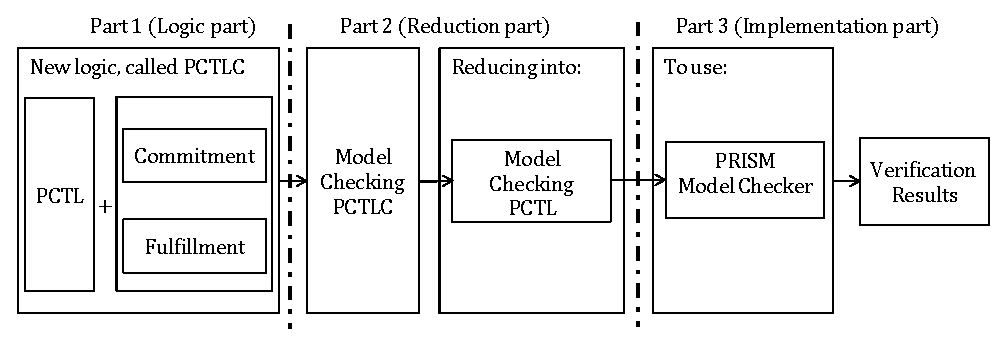
\includegraphics [width=14cm, height=5cm]{chap3/img/approach-cha3.eps}
  \caption{A schematic view of the probabilistic social commitment approach}
\label{approach-cha3}
\end{center}
\end{figure}


%%%%%%%%%%%%%%%%%%%%%%%%%%%%%%%%%%%%%%%%%%%%%%%%%%%%%%%%%%%%%%%%%%%%%%%
\section{The Probabilistic Logic of Commitments (PCTLC)}\label{sec:PCTLC}

In this section, we present a new modal logic called the probabilistic logic of commitments (PCTLC) to address probabilistic social commitments in MASs. The logic we introduce extends the probabilistic branching-time logic PCTL \cite{Hansson1994} with a commitment modality. To do so, we merge two existing logic namely PCTL \cite{Hansson1994} and CTLC \cite{Bentahar2012,El-Menshawy2013a} using the independent join technique \cite{Franceschet2004}. The independent join combines logics as they are defined in the literature. Thus, it ensures the preservation of each logic's properties in the new logic. Hereafter, we first present the syntax of our new logic, and then we define its semantics. Before going further, we define a new version of interpreted systems formalism with abilities to account for the uncertainty aspect in target MASs and to model the social interactions between communicating parties.

The PCTLC model is generated based on two extensions of the interpreted systems formalism \cite{Fagin1995} introduced in \cite{Bentahar2012,El-Menshawy2013a}, and \cite{Halpern2003,Wan2013} as discussed in Chapter \ref{cha:background}.

\begin{definition}[Models]\label{def:models}
Given a set of atomic propositions $AP = (p,q,r, \ldots)$, the
model $\mathfrak{M_1}=(S,I,\texttt{P},\{\sim_{i \rightarrow
j}\}_{{(i,j)}\in \texttt{Agt}^2},\nu)$ is a tuple where:
%
\begin{itemize}
\item  $S \subseteq L_1 \times \ldots \times L_n$ is a countable
set of all reachable global states for the system. A state $s$ is
reachable iff there exists a sequence of transitions from an
initial state to $s$ in which the probability of each transition
is greater than $0$.

\item  $I \in S$ is an initial global state for the system.


\item  $\texttt{P}:S\times S\rightarrow [0,1]$ is a total
transition probability function defined as $\texttt{P}(s,
s')=\tau(s,a^{s \rightarrow s'}, s')$ iff there exists a joint
action $a=(a_1,\ldots,a_n) \in ACT$ such that \\
$\sum_{i \in \texttt{Agt}} \tau_i(l_i(s),a^{l_i(s)\rightarrow l_i(s')},l_i(s')) > 0$ and $\sum_{s' \in S} \texttt{P}(s,s') =1$
for all $s \in S$.


\item For each pair $(i,j) \in \texttt{Agt}^2$,
$\sim_{i\rightarrow j} \subseteq S \times S$ is a social accessibility relation. $s \sim_{i\rightarrow j} s'$ is defined by the following conditions:
      %
  \begin{enumerate}
       \item $l_i(s)=l_i(s')$.
       \item $Var_i \cap Var_j \neq \emptyset$ such that $\forall x \in Var_i \cap Var_j$, we have $l^{x}_i(s)\!=\!l^{x}_j(s')$.
       \item $\forall y \in Var_j\!-\! Var_i$, we have $l^{y}_j(s)\!=\!l^{y}_j(s')$.
  \end{enumerate}
       %
  \item  $\nu : S\rightarrow 2^{AP}$ is a function valuating states with atomic propositions.
\end{itemize}
\end{definition}


\noindent Our model $\mathfrak{M_1}$ can be thought of as a labeled
state-transition system in which each transition from $s$ to $s'$
is annotated with a probability value in the matrix
$\texttt{P}$ indicating the likelihood of its occurrence
wherein the transition is assumed to take a discrete time-step.
This means that there is no notion of real time, while reasoning
about discrete time is possible through state variables keeping
track of time and counting transition steps. It is also important to
mention that every state in $\mathfrak{M_1}$ has at least one
outgoing transition to avoid deadlocks. Moreover, all
terminating/final states are modeled with a self-loop.


\vspace{0.2cm} \noindent \texttt{Computation paths}. We can unfold
the model $\mathfrak{M_1}$ into a set of paths. A path through the
model $\mathfrak{M_1}$ is a non-empty (finite or infinite) sequence
$\pi=s_0~s_1~\ldots$ of global states such that
$\texttt{P}(s_r, s_{r+1})> 0$ for all $r \geq 0$. Also,
$\pi(r)$ denotes the $(r+1)^{th}$ state of $\pi$, i.e.,
$\pi(r)=s_r$ for all $r \geq 0$.

\noindent \texttt{Probability Space}. Let $\Omega$ be a sample set
(or the set of possible outcomes of an experiment). A pair
$(\Omega,\mathrm{F})$ is said to be a \textit{sample space} if
$\mathrm{F}$ is a $\sigma$-algebra of measurable subsets of
$\Omega$, which are closed under countable union and complement
and often built from basic events called \textit{cylinders} (the
elements of $\mathrm{F}$ are called \textit{events}). A triple
$(\Omega,\mathrm{F},\mu)$ is a \textit{probability space} if
$\mu$ is a probability measure over $\mathrm{F}$, i.e., $0\leq\mu
(A)\leq 1$ for all $A\in \mathrm{F}$ such that:
%
\begin{itemize}
\item $\mu(\emptyset)=0$,
\item $\mu(\Omega) = 1$, and
\item $\mu(\bigcup_{k=1}^{\infty}A_k)=\Sigma_{k=1}^\infty \mu(A_k)$ for disjoint $A_k$.
\end{itemize}


The probability matrix $\texttt{P}$ induces a probability
space on the set of infinite paths $\Pi(s)$, which start in the
state $s$, using the cylinder construction \cite{Baier2008} as
follows. An observation of a finite path determines a basic event
(cylinder). Suppose $s = s_0$; for $\pi=s_0~s_1~\ldots~s_n$, we
define the probability measure $Prob_s \{\pi\}$ %$Prob_s^{fin}$
for the $\pi$-cylinder as follows:
%
\begin{equation}
%Prob_s^{fin}=
Prob_s \{\pi\}=
\begin{cases} 1~~~\textrm{if}~\pi~\textrm{consists~of~a~single~state}\\
{\prod_{\substack{r=0}}^{n-1} \texttt{P}(s_r,s_{r+1})~~~\textrm{otherwise.}}
 \end{cases}
\end{equation}
%
\noindent This extends to a unique measure $Prob_s$ on the set of
infinite paths $\Pi(s)$ w.r.t countable union and complement
\cite{Kwiatkowska2007}.


\subsection{Syntax of PCTLC} \label{sec:syntax-PCTLKC}


\begin{definition}[PCTLC syntax]\label{def:syntax}
Given a set of atomic propositions $AP$, the PCTLC formulae are
defined by the following BNF grammar:
%
\begin{align*}
    \varphi & ::= p~|~\neg \varphi~|~\varphi \vee \varphi~|~\mathcal{C}~|~ \mathbb{P}_{\bowtie k} (\psi)~|~\mathbb{P}_{\bowtie k}(\mathcal{C})\\
    \psi & ::=\bigcirc \varphi ~ | ~ \varphi ~U~ \varphi~|~ \varphi~ U^{\leq m} ~ \varphi \\
    \mathcal{C} & ::= C_{i\rightarrow j}\varphi ~| ~ Fu(C_{i\rightarrow j}\varphi)
\end{align*}
%
where: $p\in AP$ is an atomic proposition and $\mathbb{P}_{\bowtie
k}$ is a probabilistic operator where $\bowtie \in\{<,\leq,>,\ge\}$ and $k\in [0,1]$ is a probability bound or threshold. $m \in\mathbb{N}^+ $ is a positive integer number reflecting the maximum number of transitions needed to reach a certain state. $\varphi$ and $\psi$ are state and path formulae interpreted over the states and paths of $\mathfrak{M_1}$ respectively. The
Boolean connectives $\neg$ and $\vee$ are defined in the usual
way. Formulae $\mathcal{C}$, called social formulae, are special
state formulae in PCTLC that can express social properties using
the modal connectives $C_{i\rightarrow j}$ and $Fu(C_{i\rightarrow
j})$ standing for ``commitment'' and ``fulfillment of commitment''
respectively. $\bigcirc, U$ and $U^{\leq m}$ stand for ``next time'',
``until'' and ``bounded until'' path modal connectives respectively.

\end{definition}

\noindent The intuitive meanings of the temporal and probabilistic operators are straightforward from PCTL \cite{Jonsson1991}. $C_{i\rightarrow j}\varphi$ is read as ``agent $i$ commits towards agent $j$ that $\varphi$''. $Fu(C_{i\rightarrow j}\varphi)$ is read as ``the commitment $C_{i\rightarrow j}\varphi$ is fulfilled''. The probabilistic operator $\mathbb{P}_{\bowtie k}(\mathcal{C})$ on social formulae $\mathcal{C}$ states the degree of the commitment and the
fulfillment of the commitment: how much the agent is confident
about its commitment and fulfilling its commitment respectively.

PCTLC logic allows us to express properties like $C_{i \rightarrow j} \varphi \supset (\mathbb{P}_{\ge 0.95}(\top~U^{\leq 13}Fu(C_{i\rightarrow j}\varphi)))$ which means when a commitment about $\varphi$ is
held, then the probability that the commitment is fulfilled within
13 discrete-time steps is at least 0.95, where $\supset$ stands
for the logical implication.



\subsection{Semantics of PCTLC} \label{sec: semantics of PCTLC}

The semantics of our PCTLC is interpreted over the probabilistic model  $\mathfrak{M_1}$ which was introduced above.  Given a model $\mathfrak{M_1}=(S,\texttt{P},I,\{\sim_{i \rightarrow
j}\}_{{(i,j)}\in \texttt{Agt}^2},\nu)$, then
$(\mathfrak{M_1},s) \models \varphi$ states that ``a state $s$ in the
model $\mathfrak{M_1}$ satisfies the state formula $\varphi$,
$(\mathfrak{M_1},\pi) \models \psi$ means that ``a path $\pi$ in the
model $\mathfrak{M_1}$ satisfies the path formula $\psi$, and
$(\mathfrak{M_1},s) \models \mathbb{P}_{\bowtie k}(\psi)$ means that
``a state $s$ in the model $\mathfrak{M_1}$ satisfies
$\mathbb{P}_{\bowtie k}(\psi)$ if the probability of taking a path
from $s$ that satisfies $\psi$ is in the interval specified by
$\bowtie k$''. When the model $\mathfrak{M_1}$ is clear from the
context, we simply write the satisfaction relation $\models$ as
follows: $s \models \varphi$ and $\pi \models \psi$. Furthermore,
for a given pair $(i,j)\in \texttt{Agt}^2$ of agents, we denote
the number of accessible states $s'$ from a given state $s$ such
that $s\sim_{i\rightarrow j}s'$ by $|s\sim_{i\rightarrow j}s'|$.
The sample space of such pair of agents at $s$ is the set of
possible accessible states of $(i,j)$ at $s$ and is equal to
$|s\sim_{i\rightarrow j}s'|$. We also define $|s\models \varphi|$
as follows:

\begin{center}
$|s\models \varphi|=
\begin{cases}
1,~~~\textrm{if}~ s\models\varphi\\
0,~~~\textrm{otherwise.}
\end{cases}$
\end{center}

\begin{definition}[\textbf{Satisfaction}]\label{def:semantics-pctlc} Satisfaction of a PCTLC formula in the model $\mathfrak{M_1}$ is conductively defined as follows:


\begin{itemize}
\item For a non-probabilistic state formula:

$s\models p~~~~~~~~~~~~~~~~\emph{iff}~~p\in \nu(s);\\
s\models \varphi_1 \vee \varphi_2 ~~~~~~~\emph{iff}~~s\models \varphi_1~\textrm{or}~s \models \varphi_2; \\
s\models \neg \varphi~~~~~~~~~~~~~\emph{iff}~~s \nvDash \varphi;\\
s\models C_{i\rightarrow j}\varphi~~~~~~~~\emph{iff} ~~\forall s' \in S~\textrm{s.t.}~s \sim_{i \rightarrow j}s', \textrm{we~have}~s' \models \varphi;\\
%\textrm{we~have}~s' \models \varphi;\\
s\models Fu(C_{i\rightarrow j}\varphi) ~~\emph{iff} ~~\exists s' \in S~\textrm{s.t.}~s' \sim_{i \rightarrow j}s ~ \textrm{and}~s' \models C_{i\rightarrow j}\varphi;$


\item For a path formula:

%\vspace{-0.5cm}

 $\pi \models \bigcirc \varphi~~~~~~~~~~\emph{iff}~~\pi(1) \models \varphi; \\
 \pi \models \varphi_1~U^{\leq m}~\varphi_2~~\emph{iff}~~\exists~ k \leq m~~\textrm{s.t.}~~ \pi(k) \models \varphi_2 ~\textrm{and}~\forall i < k, \pi(i) \models \varphi_1;\\
 \pi \models \varphi_1 ~U~\varphi_2~~~~~\emph{iff}~~\exists~ m \geq 0~~\textrm{s.t.}~~\pi \models \varphi_1~U^{\leq m}~\varphi_2;$


\item For a probabilistic operator working over a path formula:

%\vspace{-0.5cm}
%\begin{align*}
 $s \models \mathbb{P}_{\bowtie k} (\psi)~~\emph{iff}~~Prob_s(\psi)\bowtie k~
\textrm{where:}~Prob_s(\psi)=Prob_s\{\pi \in \Pi(s)~|~\pi\models
\psi\};$
%\end{align*}

\item For a probabilistic operator working over a social formula,
where the set of events $\mathrm{F}$ is the set of states
satisfying a formula, and assuming that the probabilities of
accessible states from state $s$ are equally distributed:

%\begin{tabbing}
 $s\models \mathbb{P}_{\bowtie k}(C_{i\rightarrow j}\varphi)$
   ~\emph{iff}  $Prob(s \models C_{i\rightarrow j}\varphi) \bowtie \!k$, where:
%\end{tabbing}
%
\vspace{-0.4cm}
\begin{equation*}
Prob(s\models C_{i\rightarrow j}\varphi)=\frac{\sum_{s \sim_{i \rightarrow j}s'}|s'\models \varphi| }{|s \sim_{i \rightarrow j}s'| };
\end{equation*}

%\begin{tabbing}
$s\models \mathbb{P}_{\bowtie k}(Fu(C_{i\rightarrow j}\varphi))$
    ~~ \emph{iff}~ $Prob(s \models Fu(C_{i\rightarrow j}\varphi)) \bowtie k$, where:
%\end{tabbing}
%
%\vspace{-0.4cm}
%\begin{equation*}
\begin{align*}
%  Prob(s\models Fu(C_{i\rightarrow j}\varphi))\ =\frac{\sum_{s' \sim_{i \rightarrow j}s}|s'\models C_{i\rightarrow j}\varphi|}{|s' \sim_{i \rightarrow j}s| }
%
& Prob(s\models Fu(C_{i\rightarrow j}\varphi))\ = Prob_s\{\pi \in \Pi(s') ~|~ s' \sim_{i \rightarrow j}s ~\textrm{and}~ \pi = s' \ldots s ~\textrm{and}~ s' \models C_{i\rightarrow j}\varphi\}
\end{align*}
%\end{equation*}

\end{itemize}

\end{definition}

Note that, the probabilistic commitment is computed based on the number of
accessible states that satisfy the content over the whole number
of accessible states, which reflects the uncertainty of the agent
over the accessible states, so that over the commitment. On the other hand, probabilistic fulfillment is computed using the probabilistic
transitions of the path linking the commitment state to the
fulfillment state.


The following proposition is straightforward from the semantics:

\begin{proposition} \label{proposition-PCTLC}~\\
If $(\mathfrak{M_1},s)\models \mathbb{P}_{\leq0} (Fu(C_{i \rightarrow
j}\varphi))$ and $(\mathfrak{M_1},s)\models Fu(C_{i \rightarrow
j}\varphi)$, then the state $s$ is not reachable from the commitment state.
\end{proposition}

\begin{theorem}[Probabilistic and Conventional Commitments Equivalences]\label{Commitments Equivelances} ~\\

\begin{enumerate}
\item $(\mathfrak{M_1},s)\models \mathbb{P}_{\geq1} (C_{i \rightarrow
j}\varphi)$ ~~~iff~~ $(\mathfrak{M_1},s)\models C_{i \rightarrow
j}\varphi$

\item $(\mathfrak{M_1},s)\models \mathbb{P}_{\leq0} (C_{i \rightarrow
j}\varphi)$ ~~~iff~~ $(\mathfrak{M_1},s)\models C_{i \rightarrow
j}\neg \varphi$

\item $(\mathfrak{M_1},s)\models \mathbb{P}_{]0,1[} (C_{i \rightarrow
j}\varphi)$ ~~iff~~ $(\mathfrak{M_1},s)\models \neg C_{i
\rightarrow j}\neg\varphi \wedge \neg C_{i \rightarrow j}\varphi$

\end{enumerate}

\end{theorem}

\begin{proof}\hspace{-0.9cm}%$~\\$
%\begin{proof} %\hspace{-0.5cm} \\
 %In what follows, we prove the above equivalences of probabilistic and conventional commitments.

\begin{itemize}
\item First equivalence. ~\\
    $``\Longrightarrow"$. Assume $s\models \mathbb{P}_{\geq1} (C_{i \rightarrow j}\varphi)$.
    By the PCTLC semantics, it follows that $Prob(s\models C_{i\rightarrow j}\varphi)\geq1$.
    Thus,  $\frac{\sum_{s\sim_{i \rightarrow j}s'}|s'\models \varphi| }{|s\sim_{i \rightarrow j}s'|}\geq1$.
    This means that for all $s'\in S$ such that $s\sim_{i \rightarrow j}s'$, we have
    $s'\models \varphi$, and hence $s \models C_{i\rightarrow j}\varphi$. \\
    $``\Longleftarrow"$. Assume $s\models C_{i \rightarrow j}\varphi$. By the
    PCTLC semantics, it follows that for all $s'\in S$ such that $s\sim_{i \rightarrow j}s'$,
    we have $s'\models \varphi$ (i.e. all accessible states from $s$ satisfy $\varphi$).
    Consequently, $\sum_{s\sim_{i \rightarrow j}s'}|s'\models \varphi| = |s\sim_{i \rightarrow j}s'|$.
    Therefore, $\frac{\sum_{s\sim_{i \rightarrow j}s'}|s'\models \varphi| }{|s\sim_{i \rightarrow j}s'|}\geq1$
    and hence, $s\models \mathbb{P}_{\geq1} (C_{i \rightarrow j}\varphi)$.

\item Second equivalence. ~\\
    $``\Longrightarrow"$. Assume $s\models \mathbb{P}_{\leq0} (C_{i \rightarrow j}\varphi)$.
    By the PCTLC semantics, it follows that $Prob(s\models C_{i\rightarrow j}\varphi)\leq0$.
    Thus, $\frac{\sum_{s\sim_{i \rightarrow j}s'}|s'\models \varphi|}{|s\sim_{i \rightarrow j}s'|}\leq0$.
    Since the set of the accessible states from $s$ is not empty, then $\sum_{s\sim_{i \rightarrow j}s'}|s'\models \varphi|$
    must be 0 (i.e. $\varphi$ is not true in any of the accessible states). Consequently, for all $s'\in S$
    such that $s\sim_{i \rightarrow j}s'$, we have $s'\nvDash \varphi$, which means $s'\vDash \neg \varphi$.
     Hence, $s\models C_{i\rightarrow j}\neg \varphi$.~\\
%
    $``\Longleftarrow"$. Assume $s\models C_{i \rightarrow j}\neg \varphi$. By the PCTLC semantics,
    it follows that for all $s'\in S$ such that
    $s\sim_{i \rightarrow j}s'$, we have $s'\nvDash \varphi$. Since the set of the accessible states from $s$ is not empty,
    then $\frac{\sum_{s\sim_{i \rightarrow j}s'}|s'\models \varphi| }{|s\sim_{i \rightarrow j}s'|}\leq0$.
    Hence, $s\models \mathbb{P}_{\leq0} (C_{i \rightarrow j}\varphi)$.

\item Third equivalence. ~\\
    $``\Longrightarrow"$. Assume $s\models \mathbb{P}_{]0,1[} (C_{i \rightarrow j}\varphi)$. By the PCTLC semantics,
    it follows that $0< Prob(s\models C_{i\rightarrow j}\varphi)<1$. Thus,
    $0<\frac{\sum_{s\sim_{i \rightarrow j}s'}|s'\models \varphi| }{|s \sim_{i \rightarrow j}s'|}<1$.
    This means that it would never be the case that $\sum_{s\sim_{i \rightarrow j}s'}|s'\models \varphi| = |s\sim_{i \rightarrow j}s'|$
    nor $\sum_{s\sim_{i \rightarrow j}s'}|s'\models \varphi| = 0$. Consequently, there exist some $s', s'' \in S$
    such that $s\sim_{i \rightarrow j}s'$ and $s\sim_{i \rightarrow j}s''$ and $s'\models \varphi$ and $s''\models \neg \varphi$.
    Hence, it is impossible to have
    $\overline{s}\models \neg\varphi$ or $\overline{s}\models \varphi$ for all $\overline{s}\in S$
    such that $s\sim_{i \rightarrow j}\overline{s}$. Consequently,
    $s\nvDash  C_{i \rightarrow j}\neg\varphi$ and $s\nvDash  C_{i \rightarrow
    j}\varphi$. Hence $s\models \neg C_{i \rightarrow j}\neg\varphi$ and $s\models \neg C_{i \rightarrow j}\varphi$. ~\\
    %
    $``\Longleftarrow"$. Assume $s\models \neg C_{i \rightarrow j}\varphi$. By the PCTLC semantics,
    it follows that there exists $s'\in S$ such that $s\sim_{i \rightarrow j}s'$ and $s'\models \neg \varphi$.
    Consequently, it would never be the case that $s'\models \varphi$ for all $s'\in S$
    such that $s\sim_{i \rightarrow j}s'$. Therefore,
    $1>\frac{\sum_{s\sim_{i \rightarrow j}s'}|s'\models \varphi| }{|s\sim_{i \rightarrow j}s'|}$.
    Now assume $s\models \neg C_{i \rightarrow j}\neg \varphi$. Therefore, $\sum_{s\sim_{i \rightarrow j}s'}|s'\models \varphi| = 0$
    would never be he case as some accessible states should satisfy $\varphi$. %this means that $s\models \mathbb{P}_{\leq0} (C_{i \rightarrow j}\varphi)$
    %(see the proof of second equivalence above).
    Consequently,
    $\frac{\sum_{s\sim_{i \rightarrow j}s'}|s'\models \varphi| }{|s\sim_{i \rightarrow j}s'|}>0$.
    Thus, $0<\frac{\sum_{s\sim_{i \rightarrow j}s'}|s'\models \varphi| }{|s \sim_{i \rightarrow j}s'|}<1$.
    Hence, $s\models \mathbb{P}_{]0,1[} (C_{i \rightarrow
    j}\varphi)$.
\end{itemize}

\end{proof}
\vspace{0.2cm}
\begin{theorem}[Probabilistic and Conventional Fulfillment Equivalences]\label{Fulfiilemt Equivelances} ~\\

\begin{enumerate}
\item $(\mathfrak{M_1},s)\models \mathbb{P}_{>0} (Fu(C_{i \rightarrow
j}\varphi))$ iff $(\mathfrak{M_1},s)\models Fu(C_{i \rightarrow
j}\varphi)$ and $s$ is reachable from the commitment state.

\item $(\mathfrak{M_1},s)\models \mathbb{P}_{\leq0} (Fu(C_{i \rightarrow
j}\varphi))$ iff $(\mathfrak{M_1},s)\models \neg Fu(C_{i \rightarrow
j}\varphi)$ or $s$ is not reachable from the commitment state.

\end{enumerate}

\end{theorem}

\begin{proof} \hspace{0.5cm} \\
The proofs of these equivalences are direct from Proposition
\ref{proposition-PCTLC} and the above semantics.

 \end{proof}


%%%%%%%%%%%%%%%%%%%%%%%%%%%%%%%%%%%%%%%%%%%%%%%%%%%%%
\section{Model Checking PCTLC using Reduction}\label{sec:model-checking-pctlc}
%%%%%%%%%%%%%%%%%%%%%%%%%%%%%%%%%%%%%%%%%%%%%%%%%%%
When designing communicating agent-based systems that are complex,
and stochastic in nature, formal verification is generally
recognized as one of the best design support technologies, and a
valuable tool towards having efficient systems in terms of
ensuring the compliance of system design models against the given
requirements.

Given a multi-agent system represented as a probabilistic interpreted system $\mathfrak{M_1}$ and a specification $\varphi$ in PCTLC describing a desirable property, the problem of probabilistic model checking PCTLC can be defined as: 1) establishing whether or not $(\mathfrak{M_1},
I)\models \varphi$, i.e., if $I \in Sat(\varphi)$ where
$Sat(\varphi)$=$\{s\in S ~~|~~ \mathfrak{M_1},s \models \varphi \}$
is the set of states satisfying $\varphi$, 2) comparing the
probability of satisfying $\varphi$ with a probability threshold
$\bowtie k$, where $Sat(\mathbb{P}_{\bowtie k}(\varphi))=\{s\in S
~|~ Prob_s(\varphi)\bowtie k \}$, or 3) computing the probability
of $\varphi$, $(\mathfrak{M_1}, s)\models \mathbb{P}_{=?}
~(\varphi)$. Note that answers to the second and third queries can
be: (1) truth values, when the specification simply asks for a
comparison to a probability threshold, or (2) quantitative,
returning the actual probability.


\begin{figure}[!ht]
\begin{center}
\includegraphics [width=14cm, height=4.5cm]{chap3/img/reduction-process-cha3.eps}
  \caption{The proposed reduction technique of model checking PCTLC}
\label{reduction-process}
\end{center}
\end{figure}

Figure \ref{reduction-process} depicts the workflow of our
reduction technique. As mentioned before, the idea is to reduce the problem of probabilistic model checking PCTLC to the problem of probabilistic
model checking PCTL in order to be able to use the PRISM model
checker. Concretely, the proposed reduction technique consists of
two processes (see Figure \ref{reduction-process}). In the former
process, we transform our model $\mathfrak{M_1}$ into an MDP model.
MDPs are the standard models for describing systems with
probabilistic and nondeterministic behavior \cite{Rutten2004}. At
every state of an MDP, one or more actions are available, and each
action is associated with a probability distribution over the
successor states. That is, MDPs are not augmented with a unique
probability measure. Reasoning about probabilities of sets of
paths of an MDP relies on the resolution of the nondeterminism. In
order to define the semantics of such an MDP, as in
\cite{Forejt2011}, we use the notion of adversary to factor out the nondeterminism and consider the probability of some
behavior of the MDP (i.e., allowing us to place a well-defined
probability on the set of paths for each adversary). Informally,
at each step, the adversary picks an action, and then the next
state is picked according to the probability distribution
associated with the action. In this work, we focus on a special
class of adversaries called \emph{Memoryless Adversary} where the
choice of action depends only on the state and independent of what
has happened in the history (i.e., which path led to the current
state). An adversary is said to be memoryless if it always selects
the same action in a given state. The resulting adversaries are
basically DTMC models for which we can define a probability
measure over paths. The obtained DTMC models will be the input of
the PRISM model checker. In the latter process of the reduction
technique, we transform PCTLC formulae into PCTL formulae (see
Section \ref{sec:reducing-pctlc-to-pctl}).



\subsection{Transforming the Model $\mathfrak{M_1}$} \label{sec:reducing-proposed-model}

Given $\mathfrak{M_1}=(S,\texttt{P},I,\{\sim_{i \rightarrow j}\}_{{(i,j)}\in \texttt{Agt}^2},\nu)$, and a PCTLC formula $\varphi$, we define an MDP model $\mathfrak{M'_1}$ = $\mathscr{H}(\mathfrak{M_1})$ and PCTL formula $\mathscr{H}(\varphi)$ using the transformation function $\mathscr{H}$ such that $\mathfrak{M_1} \models \varphi$ iff $\mathscr{H}(\mathfrak{M_1})\models \mathscr{H}(\varphi)$.  Recall that the model $\mathfrak{M'_1}$ is an MDP model  $= (\mathbb{S}, AC, \textsf{P}_t ,I_i, L)$. Now, the model $\mathfrak{M'_1}$ can be defined using the function $\mathscr{H}$ as follows:


\begin{figure}[!htp]
\begin{center}
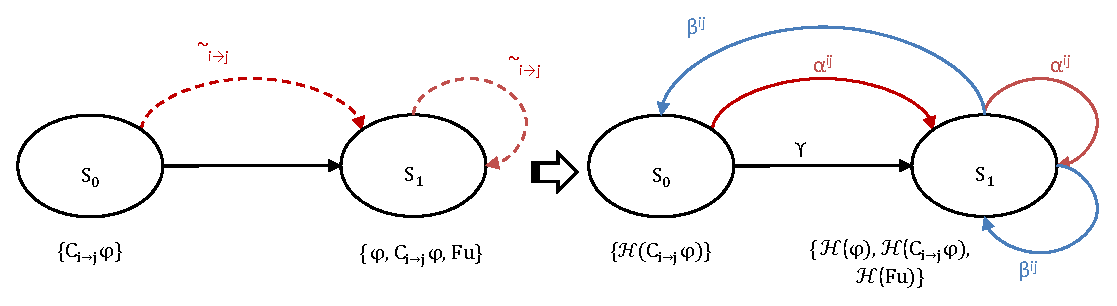
\includegraphics [width=12cm, height=4cm]{chap3/img/relation-translation.eps}
  \caption{Translating relations in $\mathfrak{M_1}$ model into actions in the MDP model}
\label{fig-relation-to-actions-cha3}
\end{center}
\end{figure}


\begin{itemize}
\item $\mathbb{S}$=$S$; $I_i$=$I$; $L$=$\nu$.

\item The set of atomic action propositions $AT$  is defined as
follows:\\
$AT = \{\varepsilon \} \cup \{\alpha_{1 \rightarrow 1},
\alpha_{1 \rightarrow 2}, \dots, \alpha_{n \rightarrow n}\} \cup
\{\beta_{1 \rightarrow 1}, \beta_{1 \rightarrow 2}, \dots,
\beta_{n \rightarrow n}\}$. Consequently, the set of actions $AC =
\{\gamma \} \cup \{\alpha^{11}, \alpha^{12}, \dots, \alpha^{nn}\}
\cup \{\beta^{11}, \beta^{12}, \dots, \beta^{nn}\}$ where $n$ is
the number of agents, $1 \leq i \leq n$, and $1 \leq j \leq n$.
Actions $\gamma, \alpha^{ij}$, and $\beta^{ij}$ denote transitions
defined, respectively, from the probabilistic transition relation
$\texttt{P}$, the accessibility relation $\sim_{i \rightarrow j}$,
and the transition added when there exists a transition labeled
with $\alpha^{ij}$ and needed to define the transformation of the
formula $Fu(C_{i \rightarrow j})$. Note that, $\varepsilon$ is the
atomic action forming $\gamma$, $\alpha_{i\rightarrow j}$ is the
atomic action forming $\alpha^{ij}$, and $\beta_{i\rightarrow j}$
is the atomic action forming $\beta^{ij}$.

\item $\textsf{P}_t$ combines the probabilistic transition
relations of $\texttt{P}$ and the probabilistic relations obtained
from translating accessibility relations $\sim_{i \rightarrow j}$
to transitions labeled with $\alpha^{ij}$ and probabilistic
transitions labeled with $\beta^{ij}$. The probability of each
transition labeled with $\alpha^{ij}$ is equal to the probability
of each other transition labeled with $\alpha^{ij}$ emanating from
the same state which is calculated by dividing one over the number
of transitions labeled with $\alpha^{ij}$ (i.e., equal
distribution). The probabilities of transitions labeled with
$\beta^{ij}$ are calculated in the same way. For states $s, s' \in
\mathbb{S}$ and action $\theta \in AC$, the function
$\textsf{P}_t$ is defined as follows:
\begin{equation*}
    \textsf{P}_t(s, \theta , s' )=
\begin{cases}
    \texttt{P}(s, s'),   & \textit{if } \theta = \gamma  \\
    \frac{1}{|s\sim_{i \rightarrow j} s'|},   & \textit{if } \theta = \alpha^{ij}\\
    \frac{1}{|s'\sim_{i \rightarrow j} s|},   & \textit{if } \theta = \beta^{ij}.
    \end{cases}
    \end{equation*}

\end{itemize}


Now, we define three different adversaries as follows: $\sigma_t$ to
be used for interpreting temporal formulae, $\sigma_c$ to be used
for interpreting commitment formulae, and $\sigma_{fu}$ to be used for
interpreting fulfillment formulae. It is worth to mention that
when defining $\sigma_c$ and $\sigma_{fu}$, some rules need to be
set. To define $\sigma_c$ at a state, action $\alpha^{ij}$ has to
be among the enabled actions at that state. Then, the memoryless
adversary $\sigma_c$ picks the action $\alpha^{ij}$ at this state,
and $\gamma$ at all other states. Meaning that, defining adversary
$\sigma_c$ at a state rather than a commitment state (the state
where $C_{i\rightarrow j}\varphi$ holds) would not be possible.
The same principle applies to $\sigma_fu$. However, $\sigma_t$
always picks action $\gamma$ at every state in
$\mathfrak{M'_1}$. The induced model of applying the adversary $\sigma$ over $\mathfrak{M'_1}$ is a DTMC model.



Hereafter, we introduce our reduction rules that translate PCTLC
formulae to PCTL formulae w.r.t a given adversary.

%%%%%%%%%%%%%%%%%%%%%%%%%%%%%%%%%%%%%%%%%%%%%%%%

\subsection{Reducing PCTLC Formulae into PCTL Formulae} \label{sec:reducing-pctlc-to-pctl}


Given the adversary $\sigma_t$, the PCTLC formulae are transformed
inductively into PCTL as follows:

$\mathscr{H}(p)=p$, if $p$ is an atomic proposition,

$\mathscr{H}(\neg \varphi)= \neg \mathscr{H} (\varphi)$,

$\mathscr{H}(\mathbb{P}_{\bowtie k}(\varphi \vee \psi))=\mathbb{P}_{\bowtie k}(\mathscr{H}(\varphi) \vee \mathscr{H}(\psi))$,

$\mathscr{H}(\mathbb{P}_{\bowtie k}\bigcirc \varphi)=\mathbb{P}_{\bowtie k} \bigcirc \mathscr{H}(\varphi)$,

$\mathscr{H}(\mathbb{P}_{\bowtie k}(\varphi~ U ~ \psi))=\mathbb{P}_{\bowtie k} (\mathscr{H}(\varphi) U \mathscr{H}(\psi))$,

$\mathscr{H}(\mathbb{P}_{\bowtie k}(\varphi~ U^{\leq m} ~ \psi))=\mathbb{P}_{\bowtie k} (\mathscr{H}(\varphi) U^{\leq m} \mathscr{H}(\psi))$,

It is important to note that, the social formulae
($C_{i\rightarrow j}, Fu$) are not transformed into PCTL by making
use of $\sigma_t$ because $\sigma_t$ does not capture the social
accessibility relation and instead it captures only the temporal
transitions at every state in the model $\mathfrak{M'_1}$.

Given the adversary $\sigma_c$, the PCTLC commitment formulae are
transformed inductively into PCTL as follows:

$\mathscr{H}(C_{i\rightarrow j}\varphi)= \mathbb{P}_{\geq 1}(\bigcirc \mathscr{H}(\varphi))$,

$\mathscr{H}(\mathbb{P}_{\bowtie k} C_{i\rightarrow j}\varphi)= \mathbb{P}_{\bowtie k}(\mathbb{P}_{\geq 1}\bigcirc\mathscr{H}(\varphi)$),


The reason behind translating a commitment formula
$C_{i\rightarrow j}\varphi$ to next operator $\bigcirc$ followed
by $\mathscr{H}(\varphi)$ is that by having transformed the social
accessibility relation $\sim_{i \rightarrow j}$ into a transition
labeled with action $\alpha^{ij}$, it is obvious that all next
states of the commitment state through the transition labeled with
$\alpha^{ij}$ satisfy $\mathscr{H}(\varphi)$ (see Figure
\ref{fig-relation-to-actions-cha3}). Hence, with respect to $\sigma_c$,
which is a DTMC model that ignores all transitions at the
commitment state except those labeled with $\alpha^{ij}$, we
clearly see that the commitment state is converted into a state
whose all successor states satisfy $\mathscr{H}(\varphi)$.

Given the adversary $\sigma_{fu}$, the PCTLC fulfillment formulae
are transformed inductively into PCTL as follows:

$\mathscr{H}(Fu(C_{i\rightarrow j}\varphi))= \mathbb{P}_{>0}(\bigcirc \mathscr{H}(C_{i\rightarrow j}\varphi))= \mathbb{P}_{>0}(\bigcirc\mathbb{P}_{\geq 1}(\bigcirc \mathscr{H}(\varphi)))$,

$\mathscr{H}(\mathbb{P}_{\bowtie k} Fu(C_{i\rightarrow j}\varphi))= \mathbb{P}_{\bowtie k} (\mathbb{P}_{>0}\bigcirc\mathscr{H}(C_{i\rightarrow j}\varphi))= \mathbb{P}_{\bowtie k}(\mathbb{P}_{>0}\bigcirc\mathbb{P}_{\geq 1}(\bigcirc \mathscr{H}(\varphi)))$.

$Fu(C_{i\rightarrow j}\varphi)$ is transformed to next operator
$\bigcirc$ followed by $\mathscr{H}(C_{i\rightarrow j}\varphi)$
because w.r.t $\sigma_{fu}$, there exists a state next to the
fulfillment state in which $\mathscr{H}(C_{i\rightarrow
j}\varphi)$ holds. Notice that the added transitions, labeled with
$\beta^{ij}$, always go from the fulfillment state to a state
where  $\mathscr{H}(C_{i\rightarrow j}\varphi)$ is satisfied (they
go either to the commitment state or to the fulfilment state
itself where in both states the formula
$\mathscr{H}(C_{i\rightarrow j}\varphi$) holds). This can be
easily seen in Figure \ref{fig-relation-to-actions-cha3}. Indeed, this
intuitively complies with the fact that for a commitment to be
fulfilled, the commitment itself has to be created before and
still alive at the moment of fulfilling it (i.e., at the
fulfillment state).
%
%
%
%It is proved that the semantic of PCTL over DTMC w.r.t adversary is the same.

%
%
\begin{theorem}[Satisfaction Equivalence]\label{Satsisfaction-Equivelance}\hspace{0.5cm} \\

Let $\sigma_t$, $\sigma_c$, and $\sigma_{fu}$ be the DTMC models
corresponding to the adversaries that capture respectively temporal formulae, commitment formulae, and fulfillment formulae. The following equivalences hold:

$(\mathfrak{M_1},s)\models p ~\text{iff}~ (\sigma_t,s) \models p$

$(\mathfrak{M_1},s)\models \neg \varphi ~\text{iff}~ (\sigma_t,s)\models\neg \mathscr{H}(\varphi)$

$(\mathfrak{M_1},s)\models \mathbb{P}_{\bowtie k}(\varphi \vee \psi)
~\text{iff}~ (\sigma_t,s) \models \mathbb{P}_{\bowtie k} \mathscr{H}(\varphi) \vee \mathbb{P}_{\bowtie k} \mathscr{H}(\psi) $

$(\mathfrak{M_1},s)\models \mathbb{P}_{\bowtie k}\bigcirc\varphi ~\text{iff}~ (\sigma_t,s) \models\mathbb{P}_{\bowtie k} \bigcirc \mathscr{H}(\varphi) $

$(\mathfrak{M_1},s)\models\mathbb{P}_{\bowtie k}(\varphi~ U ~ \psi) ~\text{iff}~ (\sigma_t,s) \models \mathbb{P}_{\bowtie k}(\mathscr{H}(\varphi)~ U ~\mathscr{H}(\psi))$

$(\mathfrak{M_1},s)\models\mathbb{P}_{\bowtie k}(\varphi~ U^{\leq m} ~ \psi) ~\text{iff}~ (\sigma_t,s) \models \mathbb{P}_{\bowtie k}(\mathscr{H}(\varphi)~ U^{\leq m} ~\mathscr{H}(\psi))$

$(\mathfrak{M_1},s)\models C_{i \rightarrow j}\varphi ~\text{iff}~ (\sigma_c,s)\models \mathbb{P}_{\geq1}(\bigcirc\mathscr{H}(\varphi))$

$(\mathfrak{M_1},s)\models \mathbb{P}_{\bowtie k}C_{i \rightarrow j}\varphi ~\text{iff}~ (\sigma_c,s) \models \mathbb{P}_{\bowtie k}(\mathbb{P}_{\geq1}(\bigcirc\mathscr{H}(\varphi)))$

$(\mathfrak{M_1},s)\models Fu(C_{i \rightarrow j}\varphi) ~\text{iff}~ (\sigma_{fu},s) \models \mathbb{P}_{>0}(\bigcirc\mathbb{P}_{\geq 1}(\bigcirc \mathscr{H}(\varphi)))$

$(\mathfrak{M_1},s)\models \mathbb{P}_{\bowtie k}Fu(C_{i \rightarrow j}\varphi) ~\text{iff}~ (\sigma_{fu},s) \models \mathbb{P}_{\bowtie k} (\mathbb{P}_{>0}(\bigcirc\mathbb{P}_{\geq 1}(\bigcirc \mathscr{H}(\varphi))))$

\end{theorem}
This theorem emphasizes that each formula has to be associated
with an adversary (i.e., a DTMC model) over which the formula can
be interpreted. The proof of the theorem with regard to PCTL
formulae is straightforward as PCTL formulae are also PCTLC
formulae. For commitment formulae, the proof is given in Theorem
\ref{soundness-PCTL} that discusses the soundness of the transformation
rules.

%
%

\begin{theorem}[Soundness and Completeness of $\mathscr{H}$]\label{soundness-PCTL}
Let $\mathfrak{M_1}$ and $\Phi$ be respectively a PCTLC model
and formula and let $\mathscr{H}(\mathfrak{M_1})$  and
$\mathscr{H}(\Phi)$ be the corresponding model and formula in
PCTL. We have $\mathfrak{M_1}\models\Phi$ iff
$\mathscr{H}(\mathfrak{M_1}) \models \mathscr{H}(\Phi)$.
\end{theorem}

%\begin{proof}$~\\$
\begin{proof} %\hspace{0.5cm} \\
Our aim here is to prove that the proposed reduction technique is
sound (i.e., the necessary condition) and complete (i.e., the sufficient condition). We prove this by induction on the structure of the formula $\Phi$. The case of PCTLC formulae that are also PCTL formulae is
straightforward. In what follows, we analyze two cases: $\Phi =
C_{i \rightarrow j} \varphi$ and $\Phi = Fu(C_{i \rightarrow j}
\varphi)$.

\begin{itemize}
\item $\Phi = C_{i \rightarrow j} \varphi$. We have
$(\mathfrak{M_1},s)\models C_{i\rightarrow j}\varphi ~\text{iff}~
(\mathfrak{M_1},s') \models \varphi$ for every $s' \in S$
such that $s\sim_{i \rightarrow j}s'$. Consequently,
$(\mathfrak{M_1},s)\models C_{i\rightarrow j}\varphi ~\text{iff}~
(\mathfrak{M'_1},s') \models \mathscr{H}(\varphi)$ for every
$s' \in \mathbb{S}$ such that $(s,\alpha^{ij},s') \in
\textsf{P}_t$. Now, w.r.t the adversary $\sigma_c$ that is defined
to interpret commitment formulae over $\mathfrak{M'_1}$,
every infinite path $\pi \in \Pi^{\sigma_c}(s)$ satisfies that
$\pi(1)=s'$ and $(\mathfrak{M'_1}^{\sigma_c},\pi(1))\models
\mathscr{H}(\varphi)$. Then,
$(\mathfrak{M'_1}^{\sigma_c},s)\models
\bigcirc\mathscr{H}(\varphi)$ for all $\pi \in \Pi^{\sigma_c}(s)$.
As the path quantifier $A$ is not defined in PCTL, and we have
$\mathbb{P}_{\geq1}$ (weaker than $A$) instead, so we obtain
$(\mathfrak{M'_1}^{\sigma_c},s)\models
\mathbb{P}_{\geq1}(\bigcirc\mathscr{H}(\varphi))$.

\item $\Phi = Fu(C_{i \rightarrow j} \varphi)$. We have
$(\mathfrak{M_1},s)\models Fu(C_{i\rightarrow j}\varphi)$ iff there
exists $s'\in S$ such that $s'\sim_{i \rightarrow j}s~
\text{and~}(\mathfrak{M_1},s')\models C_{i \rightarrow j}\varphi$.
Consequently, $(\mathfrak{M_1},s)\models Fu(C_{i\rightarrow
j}\varphi)$ iff there exists $s' \in \mathbb{S}$ such that
$(s,\beta^{ij},s') \in \textsf{P}_t$ and
$(\mathfrak{M'_1},s') \models \mathscr{H}(C_{i \rightarrow
j}\varphi)$. Now, w.r.t the adversary $\sigma_{fu}$ which is
defined to interpret fulfillment formulae over
$\mathfrak{M'_1}$, we obtain at least one infinite path $\pi
\in \Pi^{\sigma_{fu}}(s)$ that satisfies $\pi(1)=s'$ and
$(\mathfrak{M'_1}^{\sigma_{fu}},\pi(1))\models
\mathscr{H}(C_{i \rightarrow j}\varphi)$. Since $E$ is equivalent
to $\mathbb{P}_{>0}$ and $\mathscr{H}(C_{i \rightarrow j}\varphi)$
is equivalent to
$\mathbb{P}_{\geq1}(\bigcirc\mathscr{H}(\varphi))$, so we obtain
$(\mathfrak{M'_1}^{\sigma_{fu}},s)\models
\mathbb{P}_{>0}(\bigcirc\mathbb{P}_{\geq 1}(\bigcirc
\mathscr{H}(\varphi)))$.



\end{itemize}

\end{proof}


\vspace{-1.0cm}
\section{Implementation} \label{sec:implementaion PCTLC}

In this section, we apply our model checking approach on Oblivious Transfer Protocol \cite{Rivest1999}. For the purpose of providing experimental results demonstrating the effectiveness and efficiency of our reduction technique, we verify some properties of oblivious transfer protocol, expressed originally in PCTLC logic.


\subsection{Oblivious Transfer Protocol}
Oblivious transfer protocol was introduced in cryptography to
allow a sender to send some information to a receiver
in such a way that the sender remains oblivious to what is
received. We study the oblivious transfer protocol due to Rivest \cite{Rivest1999} in which the sender (Alice) has
two secret values $m_0$ and $m_1$. The receiver (Bob) would like
to know one of the two values without telling Alice which value he
learned. This protocol has been the subject of analysis for some
probabilistic properties \cite{Huang2011}. Rivest's solution uses
a trusted initializer (Ted) who participates only in the initial
setup to help both agents by providing them with some
random material. The random material includes two random strings ($r_0$ and $r_1$) ---with the same length as Alice's messages--- to be sent to Alice
in the setup phase. Then, Ted flips a bit ($d$) and sends it to
Bob along with a random string $rd$. Now, for Bob to request
$mc$ ($c=0$ or $1$), he sends Alice the bit $e=c\oplus d$
($\oplus$ is the exclusive OR logical gate: it takes as input two
bits and its output is $0$ if the two bits are equal, and $1$
otherwise). Then, Alice responds with the values $f_0=m_0\oplus
r_e$ and $f_1=m_1\oplus r_{1-e}$. Upon receiving $f_0$ and $f_1$,
Bob can compute $mc=f_c\oplus rd$. Having done so, Alice will
have no idea as to which message Bob chose, and Bob will have
learned nothing about $m_{1-c}$ (Alice's other message).

In order to use the PRISM model checker to verify and analyze
\emph{Oblivious Transfer Protocol}, the latter has to be encoded
into the PRISM input language. Simply, we treat the \emph{Sender}
(Alice) and \emph{Receiver} (Bob) in the protocol as agents. Then,
each agent is translated into a \emph{module} in the PRISM
language. Moreover, each agent is comprised of variables that
determine its local states. For example, Bob's variables are: bool
$S\_req$: send request, bool $R\_ack$: receive acknowledgement,
bit d: 0 or 1, bit c: 0 or 1, bit e: 0 or 1, bool $S\_e$: send bit
e, string $rd$: random variable obtained form Ted in the initial
setup, $R\_f$: receive $f_0$ and $f_1$. The global model is
obtained by the synchronization between all modules (agents).


\subsection{Oblivious Transfer Protocol Properties}

One of the main motivations of this chapter is to verify properties expressed as PCTLC formulae. Gurin and Pitt \cite{Guerin2002} expressed that verifying protocol properties can be performed at design time. This kind of verification aims to prove that some property will hold for all the interactions that correctly follow the protocol. Our proposed model checking technique mainly accommodates compliance by design-time verification of interaction properties. In fact, there have been various catalogs of properties proposed in the literature \cite{Bentahar2009,Cheng2006,Desai2007}. In our work, we
check \emph{safety}, \emph{Liveness}, and \emph{reachability}
properties in the Oblivious Transfer Protocol as they are popular
examples of protocol properties. These properties reflect some requirements of the oblivious transfer protocol that have to be met.

\begin{itemize}
\item \texttt{Property 1: Safety} ``Something bad will never occur".\\
This property can be generally expressed in CTL by the formula
$A\Box\neg p$ which is equivalent to $\mathbb{P}_{\geq1}(\Box\neg
p)$ in PCTLC where $p$ represents a bad situation. Such bad
situations include, for example, when Alice fulfills her
commitment of using the bit \emph{e} (received from Bob) along
with the random variables $r_0, r_1$ (obtained from Ted in the
initial setup) for calculating $f_0$ and $f_1$, but Bob does not
use the random variable $rd$ to compute his requested value
$mc$. This bad situation can be avoided using PCTLC as follows:

$\varphi_1= \mathbb{P}_{\geq1}\Box\neg[\mathbb{P}_{>0} \Diamond
Fu(C_{A\rightarrow B} (use-e))\wedge \mathbb{P}_{\geq1}\Box\neg
(use-rd)]$


\item \texttt{Property 2: Liveness} ``Something good will eventually
happen".\\
This property expresses that some good situation will eventually
occur. For example, in all computation paths it is always the case
that if Alice fulfills her commitment of using the bit $e$ and the
random strings $r_0, r_1$ for calculating and delivering $f_0$ and
$f_1$, then in all paths in the future Bob can use $f_0$ and $f_1$
to compute his requested value $mc$. This can be expressed as
follows:

$\varphi_2= \mathbb{P}_{\geq1}\Box[\mathbb{P}_{>0}\Diamond
Fu(C_{A\rightarrow B} (use-e))\supset \mathbb{P}_{\geq1}\Diamond
(comp-mc)]$


\item \texttt{Property 3: Reachability} ``Some particular situation
can be reached".\\
This property comes in the form $E\Diamond p$ which is equivalent
to $\mathbb{P}_{>0}\Diamond p$ in PCTLC where $p$ is the situation
that needs to be reached. For example, once Alice commits towards
Bob to use the bit $e$ in calculating $f_0$ and $f_1$, there
should be a possibility from the initial state for Alice to
eventually reach the fulfillment state where she can fulfill her
commitment towards Bob. This property can be expressed as
follows:

$\varphi_3= \mathbb{P}_{>0}\Diamond Fu(C_{A\rightarrow B} (use-e))$

\end{itemize}


\subsection{Experimental Results}\label{sec:experimental-results-cha3}

We have carried out 12 experiments. Our experiments were performed on a Dell laptop equipped with 32-bit Windows XP with 4 GB of RAM and Genuine Intel(R) CPU at 2.4 GHz. Table \ref{prism-results-cha3} reports the results of the performed experiments wherein (Exp.\#) denotes the experiment number, (\#Agent) denotes the number of agents, (\#States) denotes the number of reachable states, (\#Transitions) denotes the number of transitions, and (Construction Time) denotes the time needed for building the simulated model in seconds. We started our experiments with only two agents; Alice (sender) and Bob (Receiver). In this interaction, Bob requests a value
(information) from Alice and then Alice responses to Bob and sends
him the requested value in such a way that both agents respect the
rules of the protocol for encrypting and decrypting the
information.

\begin{table}%[htp]
\centering \caption{Verification results of the oblivious transfer
protocol} \label{prism-results-cha3}
\resizebox{\textwidth}{!}{ %
\begin{tabular}{|c|c|l|l|c|}
\hline
\texttt{Exp.\#} &   \texttt{\#Agents}    & \texttt{\#States} & \texttt{\#Transitions} & \texttt{Const. Time (s)}\\
\hline\hline
\texttt{Exp.1}   &\texttt{2}         &25        &75              & 0.016\\
\hline
\texttt{Exp.2}   &4       &625              &3125                & 0.047\\
\hline
\texttt{Exp.3}   &6       &$1.6*10^4$         &$1.1*10^5$        & 0.079\\
\hline
\texttt{Exp.4}   &8       &$3.9*10^5$         &$3.5*10^6$        & 0.188\\
\hline
\texttt{Exp.5}   &10      &$9.7*10^6$         &$1.1*10^8$        & 0.344\\
\hline
\texttt{Exp.6}   &12      &$2.4*10^8$         &$3.1*10^{9}$      & 0.547\\
\hline
\texttt{Exp.7}   &14      &$6.1*10^9$         &$9.2*10^{10}$     & 0.859\\
\hline
\texttt{Exp.8}   &16      &$1.5*10^{11}$      &$2.6*10^{12}$     & 1.11\\
\hline
\texttt{Exp.9}   &18      &$3.8*10^{12}$      &$7.2*10^{13}$     & 1.5\\
\hline
\texttt{Exp.10}  &20      &$9.5*10^{13}$      &$2*10^{15}$       & 2.531\\
\hline
\texttt{Exp.11}  &22      &$2.3*10^{15}$       &$5.5*10^{16}$    & 3.531\\
\hline
\texttt{Exp.12}  &24      &$6*10^{16}$        &$1.5*10^{18}$      & 5.609\\
\hline
\end{tabular}}
\end{table}

In the second experiment, we added two more agents
(receivers) who also request some values from Alice. For the rest
of the experiments, each time we add two more agents (receivers)
till we reach the maximum number of agents (24 agents) with which
we can successfully build the model.

In every experiment, we monitor the changes occurring in
(\#States), (\#Transitions), and (Construction Time) respectively.
From Table \ref{prism-results-cha3}, we notice that the state space
(represented in terms of reachable states) increases exponentially
as the number of agents increases (cf. Figure
\ref{fig:Obliviou-simulation}). Likewise, the number of
transitions also increases exponentially as more agents are added.
However, the time (in seconds) needed for building the model
increases polynomially, which shows the effectiveness of our model
checking approach when the system scales up (about $6*10^{16}$
states). The cause of this time increase in building the model
when more agents are added is that the number of reachable states
and the size of the model are increased. Moreover, the more we
become closer to the state explosion point as in experiments 20,
22, and 24, the higher time is need for building the model. This
reflects the fact that the model size in these experiments turns
out to be much bigger.

\begin{figure}%[!ht]
\begin{center}
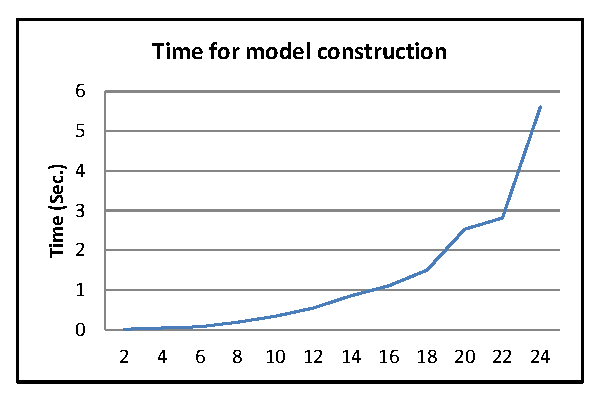
\includegraphics [width=10cm, height=6cm]{chap3/img/model-time.eps}
  \caption{Model construction time for oblivious transfer protocol}
\label{fig:Obliviou-simulation}
\end{center}
\end{figure}



It is worth noticing that starting from experiment \#2 we re-write
the desirable properties $\varphi_1$, $\varphi_2$, and $\varphi_3$
in a parameterized form, as follows ($n$ is the number of agents
in the experiment):

$\varphi_1'= \mathbb{P}_{\geq1}\Box\neg[\mathbb{P}_{>0} \Diamond
\bigwedge\limits_{i=1}^n Fu(C_{A\rightarrow B_i} (use-e_i))\wedge \mathbb{P}_{\geq1}\Box\neg
(use-rd_i)]$

$\varphi_2'= \mathbb{P}_{\geq1}\Box[\mathbb{P}_{>0}\Diamond
\bigwedge\limits_{i=1}^n Fu(C_{A\rightarrow B_i} (use-e_i))\supset \mathbb{P}_{\geq1}\Diamond
(comp-mc_i)]$

$\varphi_3'= \mathbb{P}_{>0}\Diamond \bigwedge\limits_{i=1}^n Fu(C_{A\rightarrow B_i} (use-e_i))$


However, for the purpose of model checking using our reduction
technique, every defined formula needs to be transformed according
to the reduction rules presented in Section
\ref{sec:reducing-pctlc-to-pctl}. Below we show the transformed
forms of $\varphi_1$, $\varphi_2$, and $\varphi_3$ respectively in
the case of two agents (i.e., experiment \#1).

$\mathscr{H}(\varphi_1)= \mathbb{P}_{\geq1}\Box\neg[\mathbb{P}_{>0} \Diamond \mathscr{H}(Fu(C_{A\rightarrow B} (use-e)))\wedge \mathbb{P}_{\geq1}\Box\neg \mathscr{H}(use-rd)]$.

$~~~~= \mathbb{P}_{\geq1}\Box\neg[\mathbb{P}_{>0} \Diamond(\mathbb{P}_{>0}(\bigcirc\mathbb{P}_{\geq1}(\bigcirc\mathscr{H}(use-e))))
\wedge\mathbb{P}_{\geq1}\Box\neg \mathscr{H}(use-rd)]$.


$~~~= \mathbb{P}_{\geq1}\Box\neg[\mathbb{P}_{>0} \Diamond(\mathbb{P}_{>0}(\bigcirc\mathbb{P}_{\geq1}(\bigcirc(use-e))))
\wedge\mathbb{P}_{\geq1}\Box\neg (use-rd)]$.

%%%%%%%%%%%%%%%%%%%%%%%%%%%
%%%%%%%%%%%%%%%%%%%%%%%%%%%

$\mathscr{H}(\varphi_2)= \mathbb{P}_{\geq1}\Box[\mathbb{P}_{>0}\Diamond \mathscr{H}(Fu(C_{A\rightarrow B} (use-e)))\supset \mathbb{P}_{\geq1}\Diamond \mathscr{H}(comp-mc)]$.

$~~~= \mathbb{P}_{\geq1}\Box[\mathbb{P}_{>0}\Diamond(\mathbb{P}_{>0}
(\bigcirc\mathbb{P}_{\geq1}(\bigcirc\mathscr{H}(use-e))))\supset\mathbb{P}_{\geq1}\Diamond \mathscr{H}(comp-mc)]$.

$~~~= \mathbb{P}_{\geq1}\Box[\mathbb{P}_{>0}\Diamond(\mathbb{P}_{>0}
(\bigcirc\mathbb{P}_{\geq1}(\bigcirc(use-e))))\supset\mathbb{P}_{\geq1}\Diamond (comp-mc)]$.

%%%%%%%%%%%%%%%%%%%%%%%%%%%
%%%%%%%%%%%%%%%%%%%%%%%%%%%

$\mathscr{H}(\varphi_3)= \mathbb{P}_{>0}\Diamond \mathscr{H}(Fu(C_{A\rightarrow B} (use-e)))$.

$~~~~= \mathbb{P}_{>0}\Diamond [\mathbb{P}_{>0}(\bigcirc\mathbb{P}_{\geq1}(\bigcirc\mathscr{H}(use-e)))]$.

$~~~~= \mathbb{P}_{>0}\Diamond [\mathbb{P}_{>0}(\bigcirc\mathbb{P}_{\geq1}(\bigcirc(use-e)))]$.

\noindent Table \ref{formulae-prism-results-chap3} shows the results in terms of verification time (in seconds) of model checking the above defined properties when the number of agents
varies from a simple interaction scenario of two agents to more
complicated scenarios of 24 agents. The total execution time can
be easily obtained by summing up the construction time to build
the simulated model reported in Table \ref{prism-results-cha3} and the
verification time of the considered formulae. For instance, in
Exp. 12 with 24 agents, the total execution time of verifying
$\varphi_1$, $\varphi_2$, and $\varphi_3$ is $5.609 + 2.609 +
2.453 + 2.118 = 12.789$ s.

\begin{table}%[htp]
\centering \caption{Results of model checking some properties for Oblivious Transfer Protocol} \label{formulae-prism-results-chap3}
\begin{tabular}{|c|c|c|c|c|}
\hline
\texttt{Exp.\#} &   \texttt{\#Agents}    & \texttt{Time for MC $\varphi_1$} & \texttt{Time for MC $\varphi_2$} &  \texttt{Time for MC $\varphi_3$} \\
\hline\hline
1                &2           &$<$0.001      &$<$0.001      &$<$0.001       \\
\hline
2                &4           &0.015      &0.016      &0.015       \\
\hline
3                &6           &0.032      &0.031      &0.032       \\
\hline
4                &8           &0.046      &0.047      &0.062       \\
\hline
5                &10          &0.078      &0.093      &0.078       \\
\hline
6                &12          &0.11       &0.141      &0.172       \\
\hline
7                &14          &0.203      &0.188      &0.219       \\
\hline
8                &16          &0.359      &0.328      &0.343       \\
\hline
9                &18          &0.453      &0.403      &0.5       \\
\hline
10               &20          &1.062      &0.797      &0.719       \\
\hline
11               &22          &1.813      &1.125      &1.106       \\
\hline
12               &24          &2.609      &2.453      &2.118       \\
\hline

\end{tabular}
\end{table}

Notice that the three properties hold in all conducted
experiments, meaning that our approach is successful in expressing
and verifying system  properties using PCTLC. Clearly, as depicted
in Figure \ref{fig:MC-time-properties-cha3}, the time for model
checking the three properties is similar which increases
polynomially till we reach the case of 20 agents then it grows up
dramatically. However, these results demonstrate the scalability
of our reduction-based model checking technique to verify
commitments and their fulfilments in uncertain setting for agent
communication.


\begin{figure}[!ht]
\begin{center}
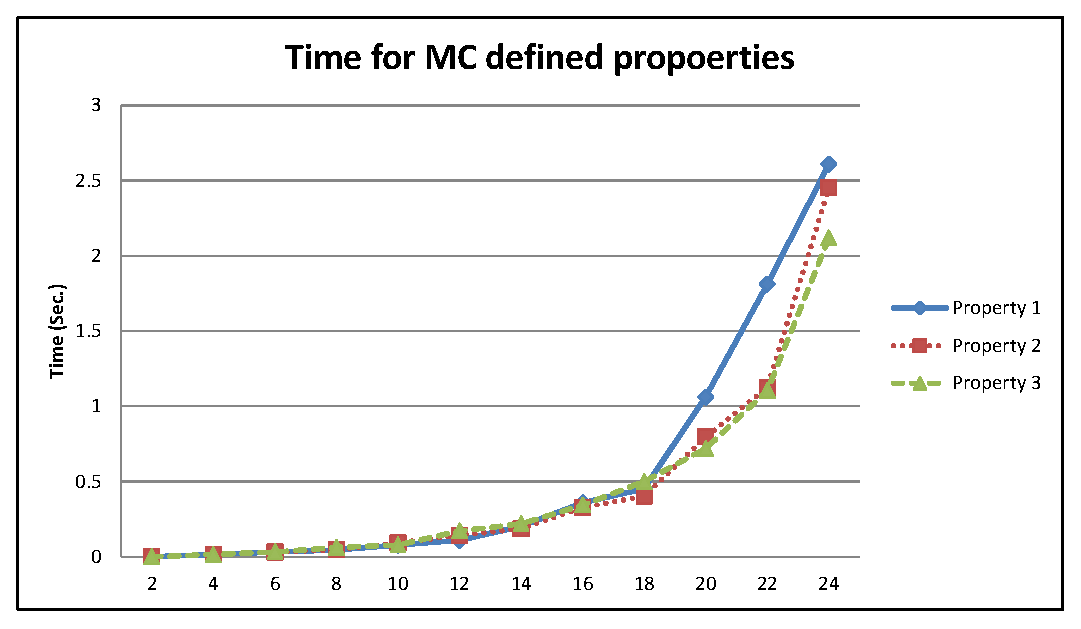
\includegraphics [width=13cm, height=7cm]{chap3/img/three-properties-time.eps}
  \caption{Time for model checking some properties for oblivious transfer protocol}
\label{fig:MC-time-properties-cha3}
\end{center}
\end{figure}

\section{Related Work} \label{sec:related-work-cha3}

The work of this chapter is related to a number of other proposals in the
literature. In this section, we give a brief overview of the most
relevant ones.

\subsection{Adding Commitment Operators to Existing Logics} \label{sec:related work Extending existing Logics}

Singh in \cite{Singh2000} extends CTL logic by adding operators for
social commitments, beliefs, and intentions in order to formally
model the interactions between interacting parties in a MAS. By
doing so, he was able to develop a specification language for
commitment-based protocols. The author defines three different
accessibility relations to intuitively capture the meaning of the
new modalities. With respect to the commitment, the author claims
that a commitment is satisfied at a certain state if and only if
the content of the commitment is true along all accessible paths
defined using an accessibility relation and emanating from the
commitment state (the state where the commitment holds). Though
the author claims that the proposed semantics is verifiable, no
concrete approach for verifying or model checking the semantics is
presented.

Bentahar and his colleagues in \cite{Bentahar2004,Bentahar2007}
present an approach that extends CTL$^*$ with an operator for
commitments and their actions, and two operators for argument and
dynamic logic respectively. To define a semantics for the
commitment modality, they present a new definition for the
accessibility relations. Moreover, their semantics is defined in
terms of the computations (paths) along which the commitment is
satisfied.

Cheng in \cite{Cheng2006} introduce a model checking method using
the SPIN model checker (Simple Promela Interpreter
\cite{Holzmann1997}) to verify commitment-based business
protocols and their compositions based on LTL logic. In this
method, commitments are not expressed directly in the logic as we
propose in our work. Instead, they are simply abstracted as
variables. Consequently, the intrinsic meaning of commitments is
not captured.

In \cite{Desai2007}, Desai and his group highlight some protocol
properties and classify them into general properties and
protocol-specific properties in order to verify the correctness of
commitment protocols. The presented properties are defined in
terms of Propositional Linear Temporal logic (LTL). Then, they
outline a technique for verifying commitment protocols and their
compositions against these properties. The proposed approach
involves using the SPIN model checker as a tool for the formal
verification. Among the general properties that they are
successfully able to verify are the deadlocks (which may result
from the contradictory between the axioms used in protocol
composition) and livelocks properties. As in \cite{Cheng2006},
commitments are simply abstracted using variables.

El-Menshawy and his colleagues in \cite{El-Menshawy2010} tried to
overcome the limitations raised in
\cite{Bentahar2004,Bentahar2007}. They propose a new logical
language called CTL$^{*sc}$ to develop a specification language
for commitment-based protocols. Their new logic extends CTL$^*$
with commitments and their associated actions. Furthermore, they
extend the temporal modalities of CTL$^*$ with past-directed
temporal modalities. The semantics of actions is not defined in a
recursive way as in \cite{Bentahar2004,Bentahar2007}, i.e., the
semantics of each action does not depend on other actions. Based
on their new logic, the authors develop a Social Negotiation
Protocol (SNP) that merges a set of dialogue games, commitment
actions and dialogue actions. Then, they present an automatic
verification technique to verify the SNP using symbolic model
checking in which they verified some given properties such as
Reachability, Safety, and Liveness. They implemented their
proposed verification technique using the NuSMV\cite{Cimatti2002}
and MCMAS\cite{Lomuscio2006} symbolic model checkers. Their
experimental results show the ability of the proposed approach to
handle large state spaces of $10^{16}$. However, the work does not
consider the uncertainty issue associated with the protocol.

In a later work, El-Menshawy et al. \cite{El-Menshawy2011a}
defined a new temporal logic called CTLC by extending CTL with
operators for social commitments and their fulfilments and
violations. In terms of defining CTLC, their main contribution is the definition of a new social accessibility relation. They define a new
accessibility relation in which they assume the existence of an
intermediate state between the commitment state and the
fulfillment state. The debtor, in their accessibility definition,
is uncertain about the current state so he looks for the
intermediate state (different from the current state) in which it
does not matter for him being in the commitment state, the
intermediate state, or the fulfillment state (i.e., the local
states of the debtor in the three global states are
indistinguishable). However, for the creditor it does not matter
being in the intermediate state or in the fulfillment state as
being in one of them is the same for him. Introducing the intermediate state makes the computation of the accessible states very complex.
The authors verified the proposed logic using a symbolic model checking algorithm they developed for this purpose.
They also extended the MCMAS model checker to be capable of
interpreting the new modalities. By so doing, they were able to
show that the problem of model checking CTLC is polynomial-time
reducible to the problem of model checking CTLK (Computation Tree
Logic of Knowledge \cite{Penczek2003}). However, the stochastic
aspect of the system being verified has not been addressed.

CTLC logic \cite{El-Menshawy2011a} has also been the focus of
El-Menshawy et al. \cite{El-Menshawy2011b,El-Menshawy2013a} and Bentahar et al. \cite{Bentahar2012} to verify and model check commitment-based protocols. In \cite{El-Menshawy2011b}, the authors investigate the use of
symbolic model checkers to verify the compliance of commitment
protocols against some given properties such as liveness and
safety. To do so, they reduce the problem of model checking CTLC
to the problem of model checking either CTLK or ARCTL (an
extension of CTL with action formulae \cite{Pecheur2006}) where
both are extensions of CTL. This allowed them to use MCMAS
(suitable for CTLK), and NuSMV (suitable for ARCTL). On the other
hand, Bentahar et al. \cite{Bentahar2012} refined CTLC by
introducing a set of shared and unshared variables so that their
extended version of interpreted systems can account for the
communication among the interacting agents. Technically, they
associate with each agent a countable set of local variables.
Then, they use those variables to represent communication channels
through which messages are sent and received.
Furthermore, they analyzed the time complexity of CTLC model
checking in explicit models such as Kripke-like structures, and
its space complexity for concurrent programs. Their proposed model
checking algorithms are implemented on top of the MCMAS model
checker. El-Menshawy et al. \cite{El-Menshawy2013a} also modified
CTLC into CTLC$^+$ that allows reasoning about communicating
commitments and their fulfilments. In their work, they introduce a
formal reduction technique to reduce the problem of model checking
CTLC$^+$ to the problem of model checking ARCTL and the problem of
model checking GCTL$^*$. This allows them to take a benefit of
existing model checkers such as the extended NuSMV symbolic model
checker (suitable for ARCTL) and the
CWB-NC~%\footnote{\url{http://www.cs.sunysb.edu/~cwb/DOWNLOADS/CWB/current/user.ps}}
automata-based model checker (suitable for GCTL$^*$). Moreover,
they analyzed the complexity of model checking CTLC$^+$ for
concurrent programs with respect to the size of such programs and
the length of the formulae and proved it to be PSPASE-complete.
Our work extends those proposals by considering the probabilistic
aspect of social commitments.

Focusing on business models, Telang and Singh \cite{Telang2012}
propose an expressive and declarative approach capable of
specifying business models at a high level of abstraction using
the notion of social commitments. In particular, they specify
business models using CTL logic, and model check operational
interactions (a set of business interactions) specified as UML
sequence diagrams. They map each model business to a temporal
logic specification based on the progression of the states of the
relevant commitments. Concretely, they capture the business model
as an aggregation of business patterns. Then, they map each
pattern to a CTL-based specification. To verify agent
interactions, the authors use the NuSMV model checker to compute
whether operational models correctly support a business model. In
this work, commitments are translated into NuSMV variables instead
of introducing a new commitment modality as we do in our proposal.

In \cite{El-Menshawy2013b}, the authors propose a new
logical-based language to specify commitment-based protocols. The
presented language is defined in terms of ACTL$^{*c}$ logic which
in turn extends CTL$^*$ with operators for social commitments and
their actions. Like in \cite{El-Menshawy2013a}, the authors also
present a formal reduction-based verification technique to
transfer the problem of model checking ACTL$^{*c}$ to the problem
of model checking GCTL$^*$. They implement their automatic
reduction-based model checking approach on top of the CWB-NC model
checker. Like in their proposal in \cite{El-Menshawy2013a}, agents
are assumed to be certain about their commitments.

In \cite{Gerard2013}, Gerard and Singh introduce an approach that
specify commitment protocols and their refinements using guarded
messages. The meaning of each message is defined as a set of
actions. They use CTL as the underlying logic in which the
specification is defined. The authors propose a model checking
technique to seek whether a protocol refines another protocol
correctly under certain conditions or not. The proposed tool
``Proton'' was implemented on top of the MCMAS model checker. The
commitments, which supposed to be certain, are modeled as objects
which are mapped into domain variables in ISPL (the input language
of MCMAS).

\subsection{Probabilistic Commitments} \label{sec:related work PC}

Uncertainty in commitments has to date received little attention by researches of MASs community. Herein, we review some existing proposals that treat commitments in the presence of uncertainty.

In \cite{Witwicki2007}, Witwicki and Durfee presented a
commitment-based methodology for approximating the optimal joint
policy in agent coordination. They proposed a technique to
decompose large mathematical programs that encodes the decision
problems of all agents into 1) a search for optimal commitments
regarding each agent's outgoing influences; and 2) a search for
optimal local policies that respect the commitments decided upon.
For a given set of commitments, they add constraints to the
traditional linear program formulation of MDPs to guarantee that a
feasible policy respects the commitments. Each agent can then
solve its linear program separately.

In another work, Witwicki and Durfee \cite{Witwicki2009}
investigated the use of probabilistic commitments in service
orientation. They proposed a commitment-based negotiation
mechanism based on uncertain durations by which service providers
agree to provide a service within a given time and certain
probability. The commitment between service providers and service
requesters use temporal and probabilistic parameters to summarize
expectations over future agent activities. Agents (providers and
requesters) then benefit from these commitments to build policies
about how to achieve (for providers) or utilize (for requesters)
these anticipated service outcomes. MDPs were adopted as the
underling models for modeling their agent-based systems. While the
semantics of the commitments was not formally described (i.e., in
term of logic), they have given a definition for the probabilistic
commitment as follows. ``A probabilistic temporal service
commitment $C_{ij}(s) = \langle t, \rho\rangle$ is a guarantee
that agent $i$ will perform (for agent $j$) the actions necessary
to deliver service $s$ by time $t$ with probability no less than
$\rho$" \cite{Witwicki2009}. By making use of these  probabilistic
commitments, agents can make promises to each other even if they
cannot fully guarantee service provision.


Unlike the proposals in \cite{Witwicki2007,Witwicki2009}, we
precisely use social commitments as a means of communication between
the interacting agents. In addition, these proposals
do not consider the verification aspect of commitments. However, we address the commitments between communicating parties from a formal perspective. That is, we integrate a commitment modality to probabilistic logic so that the verification of such commitments becomes achievable by means of model checking.


\subsection{Comparison}

We compare our work to the existing approaches by taking into
consideration the following criteria: Formalization, Uncertainty,
and Verification. Formalization reflects the use of formal logics
such as LTL, CTL, CTL$^*$, ARCTL or PCTL to represent and specify
the commitments. Uncertainty property indicates whether the
probabilistic behavior is considered or not. Finally, Verification
confirms the presentation of a formal verification technique to
verify the proposed approach. Table \ref{table:comparison1} shows
a summary about the comparison between our work and the existing
approaches based on the criteria described above.

\begin{table}
\centering \caption{Comparison between our approach for the probabilistic commitments and the related work} \label{table:comparison1}
\begin{tabular}{|c|c|c|c|}
\hline
\texttt{Approach}       & \texttt{Formal}   & \texttt{Uncertainty} & \texttt{Verification}\\
\hline
\hline
\cite{Bentahar2004,Bentahar2007,Singh2000}       & $\surd$         &   & \\
\hline
\cite{Bentahar2012,Cheng2006,Desai2007,El-Menshawy2010,El-Menshawy2011b,El-Menshawy2013a,El-Menshawy2013b,El-Menshawy2011a,Gerard2013,Telang2012}      & $\surd$         &   &$\surd$ \\
\hline
\cite{Witwicki2007,Witwicki2009}      &          &$\surd$   & \\
\hline
Ours                     &$\surd$   &$\surd$  &$\surd$    \\
\hline

\end{tabular}
\end{table}
%%%%%%%%%%%%%%%%%%%%%%%%%%%%%%%%%%%%%%%%%%%%%%%%%%%%%%%%
\begin{table}
\centering \caption{Comparison between PCTLC and existing logics in terms of the adopted logic} \label{table:comparison2}
\begin{tabular}{|c|c|c|c|c|c|c|}
\hline
\texttt{Approach}       & \texttt{LTL}   & \texttt{CTL} & \texttt{CTL$^*$} & \texttt{ARCTL}     & \texttt{PCTL} &\texttt{None}\\
\hline
\hline
\cite{Cheng2006,Desai2007}    &$\surd$          & & & & &\\
\hline
\cite{Bentahar2012,El-Menshawy2011b,El-Menshawy2013a,El-Menshawy2011a,Gerard2013,Singh2000,Telang2012}       &          &$\surd$  && && \\
\hline
\cite{Bentahar2004,Bentahar2007,El-Menshawy2010}  &          &  &$\surd$ & &&\\
\hline
\cite{El-Menshawy2013b}      &          & &  &$\surd$ &&\\
\hline
\cite{Witwicki2007,Witwicki2009}      &      &    &   && &$\surd$\\
\hline
Ours                     &   &  & & &$\surd$ & \\
\hline


\end{tabular}
\end{table}

In terms of formalization, our approach shares with most of the
surveyed proposals the idea of extending existing temporal logics
with new modalities for the commitments and their fulfilments.
However, the main feature that distinguishes it from others lies
in the logic being extended to handle social commitments. While
others adopt conventional, non-probabilistic logics such as LTL,
CTL, and CTL$^*$, ours is the only work that builds on a
probabilistic logic, namely PCTL. Table \ref{table:comparison2}
compares between our approach and other proposals with respect to
the underlying logic that has been extended to specify social
commitments.

From the verification perspective, like proposals in \cite{El-Menshawy2011b,El-Menshawy2013a,El-Menshawy2013b}, we adopt a formal reduction technique as the underlying basis for our model checking to translate the problem of model checking our logic to the problem of model checking an existing logic. However, to the best of our knowledge, non of the existing approaches has verified social commitments in the presence of uncertainty. Therefore, our approach outperforms the related approaches as it is the first attempt to  tackle the verification problem of the probabilistic social commitments. Table \ref{table:comparison3} displays a comparison between our approach and the existing ones in terms of the used model checkers.

\begin{table}
\centering \caption{Comparison between PCTLC and existing approaches in terms of the used verification tool} \label{table:comparison3}
\begin{tabular}{|c|c|c|c|c|c|c|}
\hline
\texttt{Approach}       & \texttt{SPIN}   & \texttt{MCMAS} & \texttt{NuSMV} & \texttt{CWB-NC}     & \texttt{PRISM} &\texttt{None}\\
\hline
\hline
\cite{Cheng2006,Desai2007}    &$\surd$          & & & & &\\
\hline
\cite{Bentahar2012,El-Menshawy2010,El-Menshawy2011b,El-Menshawy2011a,Gerard2013}       &          &$\surd$  && && \\
\hline
\cite{El-Menshawy2010,El-Menshawy2011b,El-Menshawy2013a,Telang2012}  &          &  &$\surd$ & &&\\
\hline
\cite{El-Menshawy2013b}      &          & &  &$\surd$ &&\\
\hline
\cite{Bentahar2004,Bentahar2007,Singh2000,Witwicki2007,Witwicki2009}      &      &    &   && &$\surd$\\
\hline
Ours                     &   &  & & &$\surd$ & \\
\hline


\end{tabular}
\end{table}




%%%%%%%%%%%%%%%%%%%%%%%%%%%%%%%%%%%%%%
\section{Summary}\label{sec:conclusion-cha3}


In this chapter, we introduced a new model checking technique for
social commitments among agents interacting in uncertain settings.
We specified properties for such systems using Probabilistic
Computation Tree Logic of Commitments (PCTLC). The PCTLC logic
extends PCTL with a social operator for commitments and their
fulfillments. Target systems are modeled using a new version of
interpreted systems which incorporates and extends two different
versions of interpreted systems formalism to capture the
probabilistic behavior of MASs, and account for the communication
between interacting entities. The proposed model checking
technique consists of a set of reduction rules to formally reduce
the problem of model checking PCTLC to the problem of model
checking PCTL so that the use of the PRISM model checker is made
possible. The proposed verification approach was evaluated through
implementing the reduction tool on top of the PRISM model checker
and then applying it on a real case study from the cryptography
domain namely the oblivious transfer protocol. The obtained
results show the effectiveness of the proposed technique. In
particular, we were successfully able to verify some desirable
properties expressed originally in PCTLC. We also showed that the
proposed reduction technique is scalable as we were able to perform the model checking for models made of up to $1.56*10^{18}$ states
and transitions.

%We showed that the system is scalable as we were able to perform the model checking using our approach for models made of up to $1.56*10^{18}$ states and transitions.
In the next chapter, we investigate how our approach for probabilistic social commitments can be exploited to handle the interaction between social commitments and agents' knowledge in MASs.


